%%%%%%%%%%%%%%%%%%%%%%%%%%%%%%%%%%%%%%%%%%%%%%%%%%%%%%%%%%%%%%%%%%%%%%%%%%%%%%%%%%
%% Formato de Edición de Artículos a ser publicados 
%% en la Revista Maskana de la Universidad de Cuenca
%% Dirección de Investigación - DIUC
% 
%
%	Versión 1.0, Octubre de 2014
% Ayuda sobre el uso de esta plantilla diríjase a kenneth.palacio@ucuenca.edu.ec
%
%
%%%%%%%%%%%%%%%%%%%%%%%%%%%%%%%%%%%%%%%%%%%%%%%%%%%%%%%%%%%%%%%%%%%%%%%%%%%%%%%%%%%

%Inicio del documento.


% Por favor no modifique el tpo de letra ni utilice otra clase diferente a la indicaca.
\documentclass[11pt]{article}

% Coloque aquí otros paquetes que pueda necesitar siempre que no entren en conflicto
% con los siguientes:
\usepackage{Maskana-template}
\usepackage{graphicx,url}
\usepackage[brazil]{babel}   
\usepackage[utf8]{inputenc}  
\usepackage{multicol}
% UTF-8 encoding is recommended by ShareLaTex     
\sloppy


% Modifique el título del artículo: utilice \\ para dividir en dos líneas.
\title{Architecture to detect patterns from bibliographical data sources }

% Edite los nombres de los autores: puede haber varios autores simplemente agréguelos.
% Un autor puede tener varias ailiaciones, sepárelas por coma; tal como se muestra para
% el tercer autor:
\author{Nombre del Primer Autor\inst{1}, Nombre del Segundo Autor\inst{2}, Nombre del Tercer Autor\inst{1,3} }

% Edite a continuación las afiliaciones de los autores:
% Indicando su departamento/unidad/grupo de investigación, universidad/centro/institución
% dirección, ciudad, país y código postal.
% Si varios autores tienen la misma afiliacion, no repita la información. 
% Para ello utilice los índices.
\address{Afiliaci\'on del primer autor, nombre de la universidad,\\
  Dirección de la Universidad, ciudad, pais, código postal
\nextinstitute
  Afiliación del segundo autor, nombre de la universidad,\\
  Dirección de la Universidad, ciudad, pais, código postal
\nextinstitute
  Afiliación del tercer autor, nombre de la universidad,\\
  Dirección de la Universidad, ciudad, pais, código postal
  \email{\{primero,segundo\}@universidad.edu, tercero@universidad2.edu}
}

%%%%%%%%%%%%%%%%%%%%%%%%%%%%%%%%%%%%%%%%%%%%%%%%%%%%%%%%%%%%%%%%%%%%%%%%%%%%%%%%%%%%%%%%%%%%%%%%%%%%%%%%%
% Inicio del documento escrito

\begin{document} 

%%%%%%%%%%%%%%%%%%%%%%%%%%%%%%%%%%%%%%%%%%%%%%%%%%%%%%%%%%%%%%%%%%%%%%%%%%%%%%%%%
% En caso que su artículo esté escrito en inglés considere:

%% Note: Use the correct words according to the language of
%% your paper, if you use English:
%Please change ``Referencias'' to ``References''
\renewcommand{\refname}{References}
%Please change ``Tabla'' by ``Table''
\renewcommand{\tablename}{Table}
%Please change ``Figura'' by ``Figure''
\renewcommand{\figurename}{Figure}
%Please change ``Agradecimientos'' by ``Acknowledgements''
\acknowName{Acknowledgements}
%%%%%%%%%%%%%%%%%%%%%%%%%%%%%%%%%%%%%%%%%%%%%%%%%%%%%%%%%%%%%%%%%%%%%%%%%%%%%%%%%%%

\maketitle

%Escriba el resumen de su artículo en inglés dentro del siguiente entorno:
\begin{abstract}
%(i) mencionar los principales objetivos y el alcance de la investigacion (lo que se hizo, por que se lo hizo y para quien se escribio el articulo?); (ii) describir los metodos empleados en la investigacion; (iii) resumir los resultados obtenidos; y (iv) mencionar las principales conclusiones derivadas de la investigacion. Los resumenes se redactan, por lo general, en tiempo pasado, porque se refiere al trabajo ya efectuado. 

%Increasingly the use of online scientific publications is more noticeable. There is an extremely large number of scientific publications in the web. For researchers its challenging pursue a topic, find peers interested in collaborate in a certain topic or review literature. We propose a novel architecture to detect patterns from different bibliographical data sources available online. We apply this architecture to find similares knowledge areas in the domain of Ecuadorian researchers using Linked Data principles.
%
Increasingly the use of online scientific publications is more noticeable. There is an extremely large number of scientific publications in the web. For researchers its challenging pursue a topic, find peers interested in collaborate in a certain topic or review literature. We propose a novel architecture to join multiple bibliography sources and detect patterns, %, support discovery and reuse of data and knowledge. 
enriching a data model using ontologies, vocabularies and Linked Data technologies. We apply this architecture to have a central repository with bibliographic resources and find similar knowledge areas in the domain of Ecuadorian researchers. 

\end{abstract}

%Escriba en inglés las palabras clave de su artículo dentro del siguiente entorno:     
\begin{keywords}
Linked Data, KDD, Ecuador.
\end{keywords}

%%% Escriba las diferentes secciones de su artículo

\section{Introduction}
\label{sec:Intro}

%Research in Iberoamerica has increased in recent years. According to the publication of the State of Science 2015 the number of items registered in the Science Citation Index (SCI)  grew by 123 \%. Increasing its participation in international databases to increase its local scientific production. One of the most prominent countries is Brazil that increased its number of publications by 2.5. However, it has several limitations, as the amount of resources invested in research in contrast to the world average. It should be noted that Latin America is the second fastest growing world after Asia \cite{Albornoz}. It has a wide range of areas of knowledge, in addition, each country has different strategic ways to address the problems of a region. Which provides a set of solutions that can be an advantage compared to first world countries in the field of research, as these solutions should be able to cope with this heterogeneity in Latin America. 

The number of publications we can access almost instantaneously is rapidly increasing through using online resources such as search engines and digital libraries. This makes it more challenging for researchers to pursue a topic, review literature, track research history because the amount of information obtained is too extensive unless the user knows the name of the exact research paper that is looking for.


%One approach of the Institutions of Higher Education (IHE) of Latin America is to contribute to the sustainable development of society through the cooperation of students and teachers, driven or promoted  by research. 
Currently, certain information about researchers and their bibliographic resources are scattered among various digital repositories, text files or bibliographic databases. When you need to propose projects with several researchers in a specific area belonging to different Institutions of Higher Education (IHE), raises questions such as: Who it works in similar lines of research? or how can you create a network of researchers in a common area when we do not know if they exist? In addition, defining the profile of a person in analysis, get their articles, know which one are the magazines that were accepted, among others, it is obligatory to access to multiple data sources. Given that, it is known that this process is manual, syntactic and different for each source of bibliographic resource available on the Web.

Expand the scope of this knowledge base will allow the entire Ecuador to have a centralized digital repository which has information of Ecuadorian researchers based in bibliographic resources. This project aims to encourage interagency collaboration and obtain as a result of this work a validated semantic repository, locate researchers working in similar research areas and provide updated information accessible and reusable. Enhancing the generation of research networks with academic peers in the region and provide greater opportunities for cooperation and collaboration to the participating institutions.

The rest of this paper is organized in the following way: section \ref{label:relatedwork} presents some related word. We outline the architecture proposed in the section \ref{label:arch}. In section \ref{label:usecase} we apply this architecture for a use case where we detect similar areas in the domain of Ecuadorian Researchers. %Results are presented in section \ref{label:results} and final 
Conclusions and future work are in section \ref{label:conlusionsfurtherwork}.

\section{Related Work}
\label{label:relatedwork}

%It is necessary to have tools that facilitate the work of researchers. in which several projects have worked. Semantic Scholar is a intelligent search engine that  utilize methods from data mining, natural-language processing, and computer vision to create powerful new searches and discover experiences. Semantic Scholar identifies connections between documents, even inside scanned ones as well as images and diagrams, based on phrases, keys, authors, topics, other data and citations \cite{semanticscholar}. Another one is GeoLink that is a smarter academic search engine that would help geoscientifics find publications and the exact data sets they want. Using linked data and Ontology design pattern-based integration in information geospatial. GeoLink's participating repositories include content from field expeditions, laboratory analyses, journal publications, conference presentations, theses/reports, and funding awards. \cite{Krisnadhi01} \cite{Krisnadhi02}.

Similar work have been achieved in the area of geoscience. The work showed in \cite{Krisnadhi2015TheGF} present Geolink project a part of EarthCube\footnote{EarthCube is a community-led cyberinfrastructure initiative for the geosciences; http://earthcube.org/}  that integrates seven repositories using Ontology Design Patterns (ODPs) \cite{Gangemi2005} defined manually. They have a set of ODPs as the overall scheme, rather than a monolithic ontology is used. To obtain data they executed federated queries. In our case all sources form a single repository and we do not use federated queries because the response time is  too long and must change every time a new data source is added. The data model Geolink is defined specifically for geodata, which it differs from our proposal covering several domains according to the bibliographic source.


The project called Semantic Schoolar have access to sources such as Arxiv, DBLP and CiteSeer  where they took publications in pdf format to extract figures, tables , and captions \cite{eps271285} and they process citations to find relationated papers, similar areas, similarity between abstracts,etc. They are trying to cover the domain of Computer Science and offer a search engine to ease the review of literature \cite{AAAIW1510092}. On other hand, we get  a bibliographic resource wich is enriched with data from other sources using Liked data Technologies.

There is a work in \cite{Alfraidi} that retrieves publications from Google Schoolar to find relationships based in the citations or references which gives an insight of the hierarchy distribution of publications around a given topic. The relationships are visualized in a 2D graph where nodes represent documents and links represent the citations or references between them. Although the user could see the papers connected in a topic or the most leading papers in the area. They can not make a network of researchers that work in a  certain area, some papers could be banned using just a source and in some areas there is a big amount of publications which can be difficult to visualize in a 2D graph. 

\section{Generic Architecture}
\label{label:arch}

In this section we present a generic architecture to use academic literature available on the web and find some kind of relationship between authors and their publications. Our approach relies on three different modules, namely: Data Extraction, Data Enrichment and Pattern Detection. The high-level modules of the architecture are illustrated in Figure \ref{fig:achitecture} and their features will be explained along this section.

 \begin{figure}[ht!]
	\centering
		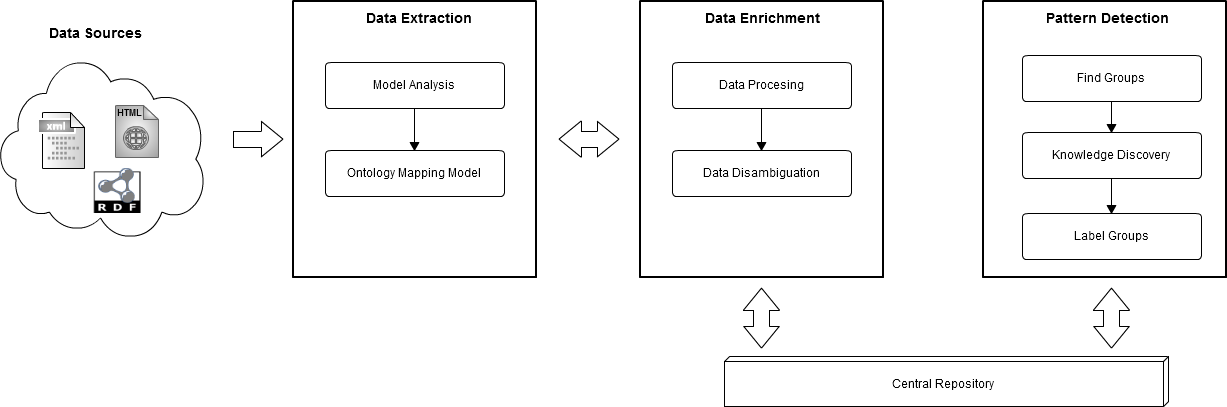
\includegraphics[height=5.2cm]{platformDiagram.png}
	\caption{General architecture to detect patterns from bibliographic data sources.}
	\label{fig:achitecture}
\end{figure}

\begin{itemize}
\item We encompass different bibliographic \emph{Data Sources}, which are heterogeneous. Access in some of this sources its limited due to the restrictions of payment, subscriptions or quota violations. We could get some descriptive information of academic literature such as title, abstract or keywords.
\item The \emph{Data Extraction} module manage heterogeneous data sources and extract it. This data is described using a bibliographic ontologie and  the \emph{Model Analysis} component analyze the structure of each model. After that, the data described is mapped in the \emph{Ontology Mapping Model} component with a common model.
\item The \emph{Data Enrichment} is the core of the system because data run through this module to be processed and stored in the \emph{Central Repository}. The main goal of this module is feed the \emph{Central Repository} with information that runs through \emph{Data Processing} component which put together all information extracted. After that, in the  \emph{Data Disambiguation} component the data is processed to remove inconsistent information.
\item The \emph{Pattern Detection} is the module which detect patterns from the data collected. Basically, the whole data is taken from the \emph{Central Repository}  that is the input for the \emph{Find Groups} component to detect some kind of association in the data set and group it. The \emph{Knowledge Discovery} component it is used to extract knowledge from the associated groups. To speed up queries and have organized groups, each group is labeled in the \emph{Label Groups} component. Finally, results are stored in the \emph{Centralized Repository} for further queries.
\end{itemize}

The modules above described have been used to join different bibliographical sources and detect similar knowledge areas in the domain of Ecuadorian researchers. In the following section we provide detailed information how we use the different modules proposed.

\section{Use case}
\label{label:usecase}

\subsection{Data Sources}
The different data sources shows in Figure \ref{fig:achitecture}  represent repositories of authors and scientific publications of different areas. In our case authors sources are distributed in different higher institutions through institutional repository DSpace\footnote{DSpace is the software of choice for academic, non-profit, and commercial organizations building open digital repositories; http://www.dspace.org}. The scientific publications  are extracted from bibliographic sources such as Microsoft Academics, Google Scholar, DBLP, Scopus, etc that make available their data via API, web pages or files. The data vary in their content either because each source has a different structure or that access to data is restricted as in the case of Scopus, which can make a maximum of 5000 querys  by ip, otherwise the source blocks access for seven days. Scopus, is characterized by data affiliation of authors, tables, graphs of publications, authors study areas, etc. While DBLP or Microsoft academics do not have. Therefore we see  that it is necessary to make a unification of these bibliographic resources with different disciplines, features structures with that feed into a central repository.

It is necessary to process the data sources referred to understand the structure and  access  of your data, these tasks are described in detail in the next subsection.



\subsection{Data Extraction.}


The \emph{data extraction} module is responsible for collecting and processing bibliographic data resources from the sources mentioned in the previous section.
The extracted data are analyzed in order to define an structure using documentation of source or web scraping techniques. The data is described and mapped to a common model, using the bibliography ontology  and Linked Data Techniques. For the development of the first prototype of the project has been selected four bibliographical databases such as Microsoft Academics, Google Scholar, Scopus, DBLP  to cover different types of databases and present a scenario in which the main problems involved in making the extraction and enrichment of bibliographic resources. Every time a new source is added, you must perform an analysis of the source model and a mapping to a common data model, these two processes are abstracted into two components described below.

\subsubsection{Model Analysis.}

The different bibliographic sources provide their own resources with a logical structure which makes the data model for each source is different having the same type of information. Bibliographic resources are not ruled by a standard or comprehensive model encompassing all properties as authors, appointments, conferences, knowledge areas, etc. Some features such as DOI, ISBN, format bibliographic references of resources are ruled by International Standard Bibliographic Description (ISBD)\cite{barbaric2014isbd}, ISO 690\footnote{ISO standard for bibliographic referencing in documents of all sorts.}. Functional Requirements for Bibliographic Records (FRBR) \cite{Edward} recommended a new approach to cataloging based on an entity-relationship model a bibliographic resource. However it is not enough if we need a common data model to facilitate the processing of scientific publications.

In Figure \ref{fig:ModelMaSO} you can see the data model between two bibliographic databases: Microsoft Academics and Springer Open Access API  that represent the diversity of models of data between bibliographic databases. This heterogeneity of models represents the challenge of integrating various sources, taking into account that some sources don not publish your data model. Therefore before adding a new data source to the architecture must perform an analysis of its structure with respect to models already being used for the purpose of assigning correspondences between new source model   and model common data. \begin{figure}[ht!]
	\centering
		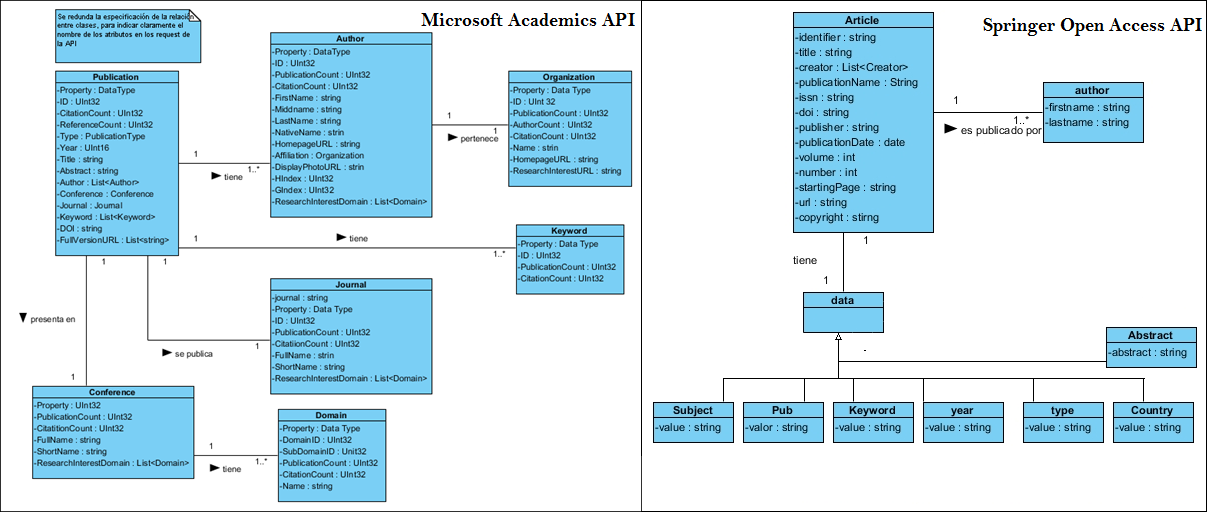
\includegraphics[height=5.2cm]{modelosMA_Springer.png}
	\caption{Data Models of Microsoft Academics API and Springer Open Access API.}
	\label{fig:ModelMaSO}
\end{figure}

In some cases an source do not publish your model data, then we use works that describe an model, form example \cite{ley2009dblp} have described the model data of DBLP. Another form is make xml requests sending as parameters the author names to source for  inquire into  data structure. The result of this component is data with defined model, after is mapped to a common model that described below.

\subsubsection{Mapping Ontology Model.}

In this component we have each data source with a different model that through a process of \emph{Mapping Model Ontology} the data  is structured in an common data model illustrated in the Figure \ref{fig:CommonDataModel}. This component find a correspondence between the properties of  source model and an common data model is using techniques of \emph{Metrics Similarity} \cite{Charikar2002SimilarityET}. This models are annotated using RDF\footnote{Resource Description Framework; https://www.w3.org/RDF/}  with an structure based in triples. This process of mapping is manual because the diversity of structures of source data models, in \cite{Ortiz} have a prototype about of a platform to automatic semantic annotation of RESTful Web services that we can use to do automatic annotation of services that offer the bibliography databases, this process is consider in a future work.

The common model proposed is described using ontology (BIBO)\cite{Frederick}, which is an ontology is used to describe bibliographic entities as books, magazines, etc. The authors are described using ontology FOAF (Friend of a Friend), it is an ontology used to describe people, their activities and their relationships with other people and objects \cite{brickley2012foaf}. 

 \begin{figure}[ht!]
	\centering
		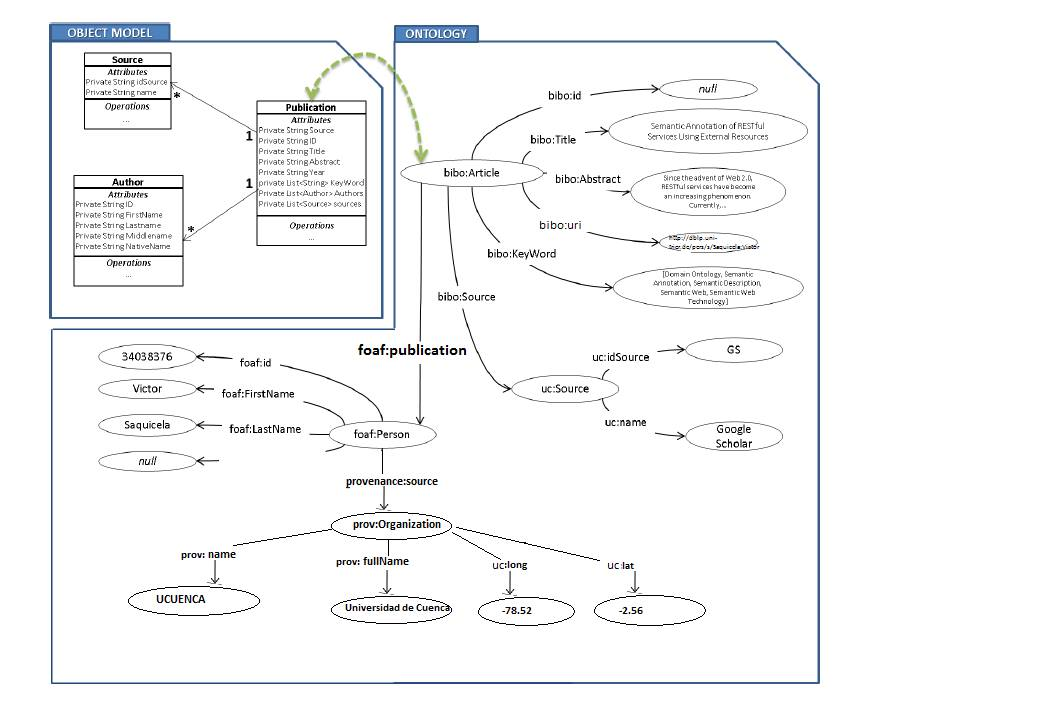
\includegraphics[height=9cm]{dataModelCommon.png}
	\caption{Common data model publications.}
	\label{fig:CommonDataModel}
\end{figure}

The data that we have has repeat entities and it is  ambiguous  determine  publications assigned to an author, in some cases author attributes are similar. So the data must be processed to be then stored, which is detailed below.
\subsection{Data Enrichment}

The module of \emph{Data Enrichment} unifies all data of publications and authors in a central repository using ontologies. We find characteristics between publications and authors assignment correspondences through a component of \emph{Data Process}. We have various entities of a same author or publication and this represent a problem of inconsistency, for this reason we have an component called \emph{Data Disambiguation} that solve this problem which is described below.

We decide that is necessary to have materialized data authors and publications in a repository to find correspondences between these locally, other option is to recover the publications at the time that an user needed. The time between making a request to an external source and the mapping takes an average of twenty seconds. Therefore we have a unit repository  to offer high availability and speed bibliographic resources to consult the publications of a specific author using SPARQL Endpoints\footnote{Services that accept SPARQL queries and return results}.

\subsection{Data Disambiguation}

The \emph{Data Extracted} module have repeated publications from different sources or publications assigned erroneously. Is necessary discover that authors are the same entity between our various sources. The prototype developed allows  define a single record of an author in a central repository using characteristics of the author and characteristics of their publications, taking advantage of ontological descriptions and algorithms similarity metrics. We have defined a priority among bibliographical sources according to the quality of the data. For example the most reliable source is Scopus, because
because it is consistent to searches such as   \textit{Juan Pablo Carvallo Vega} and \textit{Juan Pablo Carvallo Ochoa}, identifying in most cases the difference. Other data sources such as DBLP not keep complete records of the author and only use the first name and lastname, causing scientific publications are assigned to other authors.


In the component \emph{Data Disambiguation} handles the problem of data inconsistency, using the authors publications in our repository and publications the source returns, if correspondences between them are states that there is consistency between authors and their publications, this process is illustrated in Figure \ref{fig:DisambiguationProcess} also this component helps us when we need to add new publications of an author. The work present in \cite{varadharajalu2011author} have an algorithm to disambiguation using the affiliation, email, Url, Organization, Co-Authors, etc. Making in context disambiguate authors and publications. In our case  is necessary to have more information about the author to can extend the disambiguation algorithm and can desert resources that don have a relation.


\begin{figure}[ht!]
	\centering
		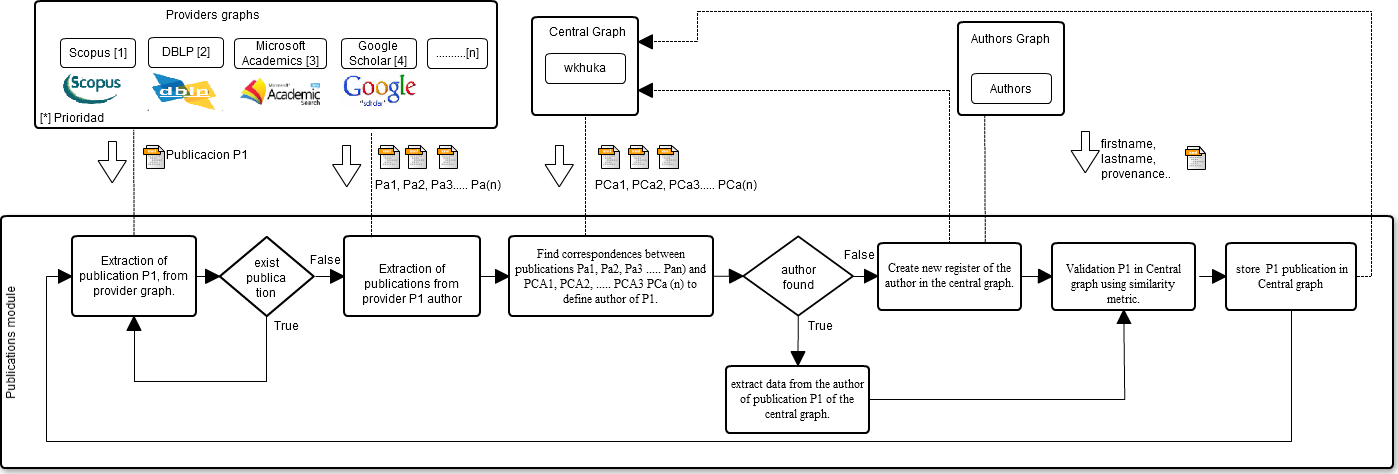
\includegraphics[height=5.2cm]{desambiguationProcess.png}
	\caption{Disambiguation Process.}
	\label{fig:DisambiguationProcess}
\end{figure}

Until now we have a central repository using Ontologies and Linked Data but it is necessary to extract knowledge from this data. In the following section we show how the pattern detection module was applied to detect similar areas between researchers. 

  
\subsection{Pattern Detection}
\label{label:detectsimilarareas}

In this section, we outline the three components of the module to detect patterns in the data stored. It uses Apache Mahout to execute algorithms of machine learning. We choose mahout for the ability to deal with massive datasets, it is a scalable Java library and we could profit of the distributed computation, because it is built upon Apache Hadoop. The whole implementation is open sourced and available on our GitHub repository\footnote{\url{https://github.com/cuent/kodar.git}}. 
%In this section, we outline a web service built to detect patterns in the data stored. The service has been called KODAR that means ``Knowledge Discovery Of Research Areas'' with the words a little bit jumbled. It uses Apache Mahout to execute algorithms of machine learning. We choose mahout for the ability to deal with massive datasets, it is a scalable Java library and we could profit of the distributed computation, because it is built upon Apache Hadoop. KODAR it is built to support the three components of the module. The whole implementation is open sourced and available on our GitHub repository\footnote{\url{https://github.com/cuent/kodar.git}}. 


\subsubsection{Find Groups}
\label{label:discoversimareas}

Broadly, keywords of academic literature talk about a certain topic area or methodology. Detecting similar areas based in the keywords . It could help us to detect researchers with interests in common and open up an opportunity to generate new research projects. Boosting interagency collaborative work and form cooperative research groups.

Firstly, we disjoin our data stored in the \emph{Central Repository}, because we just need to process the keywords to group the most common areas. Other fields such as author or title of the publication are stored in a separate file. Both files are converted in a specific Hadoop file format that is SequenceFile\footnote{Mahout also use Sequence files to manage input and outputs of MapReduce and store temporary files.}. Those files stores key/value pairs, where in the first file the key is a unique identifier and a bunch of keywords that belongs to a paper are stored as a value. Same happens in the second file with the difference in the value pair that stores the remaining fields such as author and publication. 

We use techniques of text clustering \cite{Andrews} for the \emph{find groups} module. Before to clustering the data into Mahout It is necessary to do some procedures . Data has been preprocessed to convert text in numerical values, but not all the keywords have the same relevance. The weighting technique used to magnify the most important words is Term frequency-inverse document frequency (TF-IDF). The weighted values are used to generate the Vector Space Model (VSM) where words are dimensions. The problem with this VSM generated is that words are entirely independent each other and it is not always true. Sometimes words have some kind of dependency such as \emph{Semantic} with \emph{Web}. In order to achieve this dependency we use collocations \cite{Manning}. At the time of writing, we are executing our experiment using bi-grams and an Euclidean norm (2-norm), which can change. In future experiments, it will be interesting to generate vectors using Latent Semantic Indexing (LSI) or apply a log-likelihood to take words that mostly have the chance to go together. So in the long run, we have our vectors completed to start clustering.

We start with the vectors generated to execute K-Means algorithm in Mahout. It was executed using a Cosine distance measure as the similarity measure. RandomSeedGenerator\footnote{It is used to generate random centroids} was used to seed the initial centroids. The experiment were set to 100 maximum of interations and the value of k varies according to the number of data extracted from the different bibliographic databases. Once the algorithm finishes we have our similar areas based in a bunch of keywords. The dilemma its how to detect researchers networks using the group of keywords generated, this work its done in the following section.


\subsubsection{Knowledge Discovery}

Once detected the groups of similar areas. We could extract some knowledge from the groups stablished such as what researchers could be interested to work together based in the areas they are working on. 

We have developed a MapReduce model to accomplish it as you can observe in the Figure \ref{fig:mapreducemodel}. First, we sort our vectors accord to a unique identifier. After that we merge each vector clustered with their original keyword. In our final job, we merge the resulting file of the first stage (Sort \& Join) and the additional file containing the remaining fields (title, author). Then, we get a file with all the original fields, plus a field showing the cluster that each row belongs.

\begin{figure}[ht!]
	\centering
		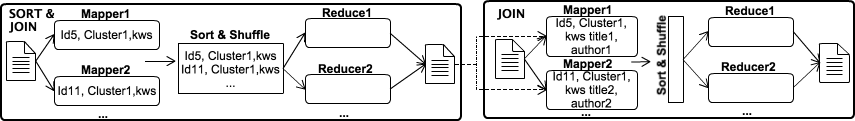
\includegraphics[height=2.295cm]{findka.png}
	\caption{MapReduce model}
	\label{fig:mapreducemodel}
\end{figure}

There is an association between authors and their publications in each group. Our next step is know what a group is about. So in the next section, we label each cluster according with their keywords.

\subsubsection{Label Groups}

Search engines could increase performance in searches by finding a general topic area based in the words that belongs to a cluster. We can respond to specific queries (i.e.: show all researchers working in a specific area or all subareas belonging to a general topic area).

We use WordNet\footnote{It is a lexical database for the English language that is used for text analysis applications.} \cite{Miller} to find synonyms, hypernyms, hyponyms and the concept of a word for all keywords in a cluster. It helps to find a common meaning in the way that words could occur together and find similar meanings. In other words, with the group of word set up we could find a concept or a topic for each cluster.

We applied Collapsed Variational Bayes (CVB) algorithm \cite{Blei} that is an implementation for Latent Dirichlet Allocation (LDA) in Mahout. We use all the words generated by WordNet plus the title and keywords of each publication to find a broader topic based in multiple subtopics described by the keywords. We use Mahout RowId to convert Term Frequency (TF) vectors into a matrix. The CVB algorithm was executed with the following parameters: 1 for the number of latent topics and 20 maximum interactions. This job is applied to each cluster.

Results are imported in the Central Repository usign RDF. Figure \ref{fig:descriptionrdf} shows the concepts and relationships used to export the results. The full arrow symbolize a relationship between classes and the dash arrow symbolize a common relationship.

\begin{figure}[ht!]
	\centering
		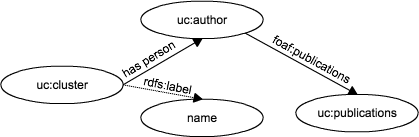
\includegraphics[height=2.9cm]{anotacion.png}
	\caption{Concepts and relationships of RDF file.}
	\label{fig:descriptionrdf}
\end{figure}

%\section{Results}
%\label{label:results}

%In the process of extraction scientific publications we use only the names of the author, for searches of publications, which generates erroneous information for example people with the same name but that  do not work on the same subject. The solution for this problem  is proposed as future work to establish a better partnership between publications and authors, so you can discern whether a publication is linked to the research of a particular author, in otherwise discard this data, improving the quality of information platform.

%After the integration and extraction we have a centralized semantic repository. Table \ref{table:statistics} show some statistics.


%\begin{table}[htbp]
%\begin{center}
%\begin{tabular}{|l|l|l|l|}
%\hline
%Bibliographic database & Publications & Authors &  Publications/authors \\
%\hline \hline
%Microsoft Academics & 3663  & 375 & 9.77 \\ \hline
%DBLP & 21433 & 1698 &  12.62 \\ \hline
%Scopus &  1134 & 136 & 8.33 \\ \hline
%Google Scholar & 367 & 47 & 7.80 \\ \hline
%\end{tabular}
%\caption{Tabla muy sencilla.}
%\label{tabla:sencilla}
%\end{center}
%\end{table}



%We are going to show the interpretation of a taken sample cluster  as result\footnote{All results can be analyzed on the web platform: \url{http://investiguemosjuntos.cedia.org.ec}}. We find that all the words listed below belongs to the general topic area of \emph{physics}. Researchers that are working in the areas listed of physics are \emph{Fern\'andez Tapia, Jaime E, Torres Arteaga, Christian Alejandro} and \emph{Aguilar Romero, Gino}. At last, a research project could be proposed with people that are working in similar areas. 

%\begin{multicols}{2}
%    \begin{itemize}
%	\item Inelastic Scattering
%	\item Flow Measurement
%	\item High Energy
%	\item Fourier Coefficient
%	\item Bose Einstein Correlations
%	\item Monte Carlo
%	\item Three Dimensional
%	\item Center of Mass
%	\item Large Hadron Collider
%	\item Charged Particles
%	\item Correlation Function
%	\item Proton Proton
%	\item Particle Physics
%	\item Experience Repor
%	\item Elliptic Flow
%	\item Heavy Ion Collision
%	\item Particle Production
%	\item Particle Emission
%    \end{itemize}
%\end{multicols}


\section{Conclusion and Further Work}
\label{label:conlusionsfurtherwork}
We have presented architecture that have a central repository with rich data from various bibliographic sources with a data model defined and described using ontologies that includes links to other data in other repositories. 


%%%%%%%%%%%%%%%%%%%%%%%%%%%%%%%%%%%%%%%%%%%%%%%%%%%%
%% Sección de Agradecimientos / Reconocimientos
%% Opcional - Se puede eliminar por completo en caso
%% que su artículo no requiera de la misma.

\begin{acknowledgements} 
  En esta sección se agradece de manera cortés por la ayuda: científica, de redacción y 
técnica (equipo y otros materiales especiales) recibida de cualquier persona o institución. Además, en 
esta sección se expresa también un reconocimiento por la ayuda financiera externa (como 
subvenciones, contratos o becas) recibida tanto para la realización de la investigación como para la 
preparación del artículo. Debe ser breve.
\end{acknowledgements}



\bibliographystyle{MaskanaStyle}
\bibliography{MaskanaBIB}

\end{document}
